\chapter{Contextual and Spatial Information in V1 Responses}
\label{chapterlabel4}
In previous chapter, the mice behaviour validates that mice can learn a complex visual navigation task with identical landmarks and can distinguish the two visual environments with identical landmarks at various positions and contexts. As described in chapter 2, the neuropixel recordings in V1 provide a rich dataset in how V1 neurons respond to visual landmarks in the dynamically changing environments. In previous study, spatial modulation is present when animal travels in a VR designed similar as the familiar environment used in training and the spatial modulation is stronger over days of contact with the VR environment. In the recordings, a novel environment is introduced with new sets of identical landmarks at same locations but also with a set of plaid landmarks shared between the familiar and novel environments. Hence, each environment contains two sets of identical landmarks which raises the question of whether the spatial modulation is a phenomenon present in particular visual patterns or in all visual patterns. When it comes to shared visual landmarks in two environments, do neurons with spatial modulation to these plaids have different behaviour in the two environment to the same visual landmarks? This chapter aims to characterise the V1 responses in the two spatial contexts by first replicating the spatial modulation found in V1 and exploring if spatial context has impact on visual responses in V1.

\section{Method}
\subsection{Spatial Binning of Visual Response}
The spike events after spike sorting are binned into a firing rate temporal vector at 60Hz aligned to the clock of the electrophysiology recording system (see chapter 2 for more details). The temporal vector is smoothed with a 200 ms window Gaussian filter. The smoothed temporal vector is further binned at 1 cm into a N \(neuron \times L lap \times P\) spatial bins matrix. When a shift of X ms is applied to the data, for example 200 ms, the temporal vector is first shifted forward by 12 time bins at 60Hz in this case. 

For \(speed \times position \) binning, the same temporal vector is used to bin at corresponding speed and position, and the temporal vector is shifted by X ms if a shift is used.

\subsection{Landmark Tuning}
The distance between landmarks is relatively small. Therefore, finding if a nueron is tuned to a landmark requires assumption about the response location is near the landmark and the response. In extreme case, binocular zone neurons can see the landmarks 20 cm ahead of the peripheral neurons and the distance between the landmarks is 20 cm. In addition, the VR has rapid change in spatial frequency of the landmarks when the landmarks are in the binocular zone and the view distance is restrained to 21cm which means that the central part of the binocular zone does not show any landmark on the screen. Taken together, the following landmark tuning method is only applied to neurons with a receptive field outside the binocular zone. Binocular zone neurons are not included in this chapter. 

Most peripheral neurons have landmark responses within 10 cm of the landmarks no matter if a temporal shift is applied (see Fig 4.1B-C and Fig 4.2B-C). The response of a neruon are binned at 5 cm bin size first and the peaks and their locations are found by Matlab function findpeaks(). A search window for each landmark is applied to the response locations, for example, the plaids would have a search window at \([60,80] \cup [100,120]\) cm. The responses are further binned at 1 cm and the exact peak values and peak locations are found within the search window. The neuron is considered to be tuned to a landmark if the response is 2 standard deviation from the baseline and the baseline is the median of the [150,170] cm positions outside of the VR. The single lap responses are extracted from the same search zone but with a lap-dependent peak location.

\subsection{Spatial Modulation Index}
Previous spatial  modulation index in Diamenti et al 2021 is finding the maximum response location along the VR from odd laps and use the responses at the same location from even laps. This peak response location is called preferred location and 40 cm before or after this location is the non-preferred location. The spatial modulation index is calculated by \(SMI_{even} = \frac{R_{even , prefer} - R_{even , nonprefer}}{R_{even,prefer} + R_{even,nonprefer}}\). This method works well in a symmetrical environment and ignore the other set of landmarks with weaker responses. In my experiments' VR setting, there are 5-6 landmarks and the first landmark's response location can make it more difficult to define what zone to search for a maximum response. Therefore, the single lap responses to each landmarks are used to calculate the landmark-specific spatial modulation index. For each landmark, the same equation \(SMI_{even} = \frac{R_{even , prefer} - R_{even , nonprefer}}{R_{even,prefer} + R_{even,nonprefer}}\) is used on neurons that are tuned to the landmark and the SMI of the odd lap peaks by even lap locations is also calculated to find the average of odd and even laps SMI values \(SMI = \frac{SMI_{odd}+SMI_{even}}{2}\).

\subsection{ANOVA Tests}
For all landmarks, the single trial responses to each of the landmark from landmark tuning method are used to run any statistical tests, ANOVA in this case. For finding if a neuron has different responses to the same landmark at the two positions, a one-way ANOVA is applied to response sets of each set of landmark which is equivalent to a t-test.

For the plaid landmarks that are shared between the two VR environments, a two-way repeated measures ANOVA is applied. The two positions of the plaids are identical on the two environments and they happen on the same lap. Hence, the two positions are repeated measures. The two way test is context (track 1 or track 2), position (position 1 and position 2), and the interaction of the two variables.

\section{Results}
\subsection{V1 Neurons Have Diverse Tuning to the Visual Features in VR}
V1 neurons have diverse responses to the sets of the visual landmarks. The labeling of the landmarks in the neural responses is illustrated in Fig 4.1A. There are 2-3 sets of identical landmarks in each environment and one set of landmarks is shared between the two environments. A purely visual neuron is expected to respond the same to the same landmark at different locations. In Fig 4.1B, raster plots across track 1 and track 2 for example neurons are shown and below them are the mean firing rate across laps in each environment. First neuron in Fig 4.1B shows the same responses to the plaid landmark at the same location in both track 1 and track 2 and the neuron has different response profiles to the first set of identical landmarks in the two tracks. In addition, this neuron shows different responses to the same plaids at the two positions in both tracks. Hence, this neuron transfers the same spatial modulation when the animal is in the novel environment. The second third and fourth example neurons in Fig 4.1B show responses to multiple landmarks across the two environments. These tuning profiles require more quantitative methods to compare how these neurons behave in the two environments. In addition, there are also many neurons similar as the third example neuron in Fig 4.1B that they have very little response to the shared plaid landmarks but also show very response profiles to the same landmarks in the two environments - this neuron has higher firing rate to the second landmark than the fourth landmark but the opposite in track 2 where the landmarks have different visual features. In Fig 4.1C, all neurons from all sessions with stable firing and significant response (95\% shuffle) within the track (see chapter 2 method for detailed criteria) are arranged by the odd laps' average peak firing position and the normalised average responses are from the even laps which shows that these V1 neurons have high stability. The familiar and novel environments are sorted by their own odd laps. From the population map across sessions, neurons within the zone of identical landmarks have side bands of responses to the same landmarks 40 cm away from the peak and some of these neurons have weaker responses to the side bands of the same visual landmarks indicating a subpopulation of neurons have spatial modulations. The example neurons in Fig 4.1B are also labelled by shapes on the side of the population maps. In the previous spatial modulation experiment design, the landmarks are arranged in completely identical repeats. However, the current design contains cue landmarks at the beginning for both environments and another landmark at the end of the novel environment. There are also large number of neurons dominated by these cue landmarks but in future analysis, the focus will be on each set of identical landmarks in the two environments. 
\begin{figure}
    \centering
    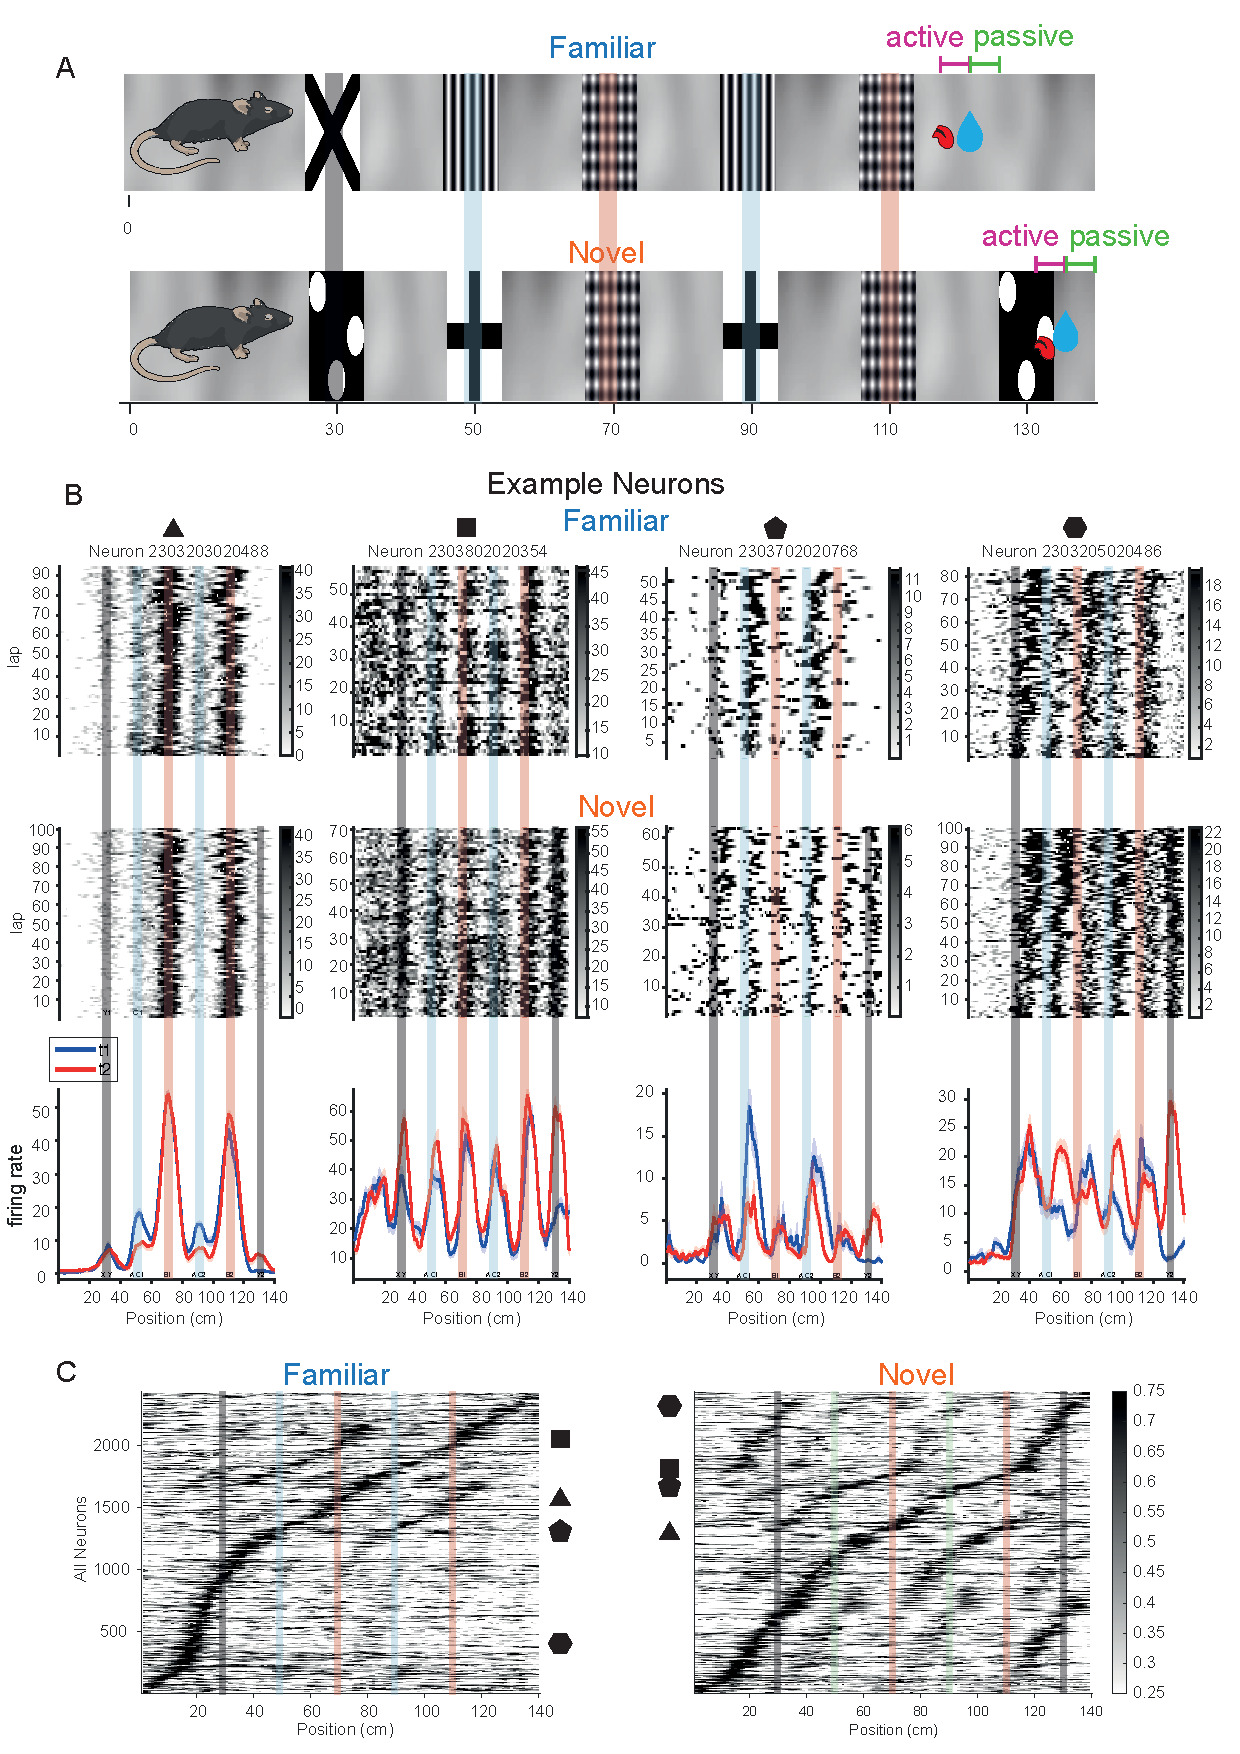
\includegraphics[width=1\linewidth]{figures//Chapter 4 V1/fig1_VR_setup_and_responses.pdf}
    \caption{A summary of visual responses in the two VR environments sorted by position and examples neurons' tuning PSTH.}
    \label{fig:population map}
\end{figure}


\subsection{Visual Response Delay Impacts Spatial Binning}
Visual responses in V1 have delays and can be impacted by the animal's running behaviour when binning the spiking activity into spatial bins in the VR. Visual responses to stimuli have a onset delay of 40-60 ms and reach the peak around 70-120 ms in V1 in the checkerboard stimuli during the same recordings and from literature in both mice and primates. When mouse runs at a high speed, for example 30 cm/s, the landmark reaches the receptive field of a neuron at position 30 cm and elicits a response, the response happens 100 ms later and the distance mouse traveled is 30 * 0.1 = 3 cm ( Fig 4.2 A). If the mouse runs at very different speed at each lap, the mean firing rates of a neuron to the landmarks can be impacted by peak responses being located at various positions. Hence, if a mouse runs in different patterns at the two positions of the identical landmarks, the difference between average response profiles can be caused simply by the running speed profiles. To show this effect, the response profiles are binned by \(speed \times position\) in Fig 4.2B. In the left panel, a neuron's response profile along the VR sorted by the mouse's running speed in the Y axis and the responses positions to the landmarks are much later at high speed than low speed. Therefore, a shift in spike onset of the neuron in the time series of the recordings is applied to cancel the visual response latency onset (Fig 4.2A shows a demonstration of the impact of applying a shift to cancel the visual response onset latency). Fig 4.2B shows the effects of applying a shift of 200 ms and 400 ms and 200 ms makes the delay impact on spatial positions almost disappear whereas 400 ms shift makes the responses at high speed happen at earlier position than responses at low speed. In Fig 4.2 C-D, on the left hand side is the spatial binning of both environments with no shift applied for two example neurons (top neuron is the same neuron as Fig 4.2C) and the right hand side is spatial binning after applying a 200 ms forward shift on two example neurons. In the raster plots, the response peak locations are more aligned together across laps. In the average responses of the two example neurons, both the locations of the responses are more shifted towards the original landmark locations (forward) and the ressponse peaks are sharper. In the second example neuron at the bottom, responses are dominated by the shared plaid landmarks. Applying a shift makes this neuron's responses to these shared plaid landmarks more comparable across the two tracks where the response patterns to the two plaids at 70 cm and 110 cm are almost identical in the two tracks with the shift. Overall, this method finds that applying a 200 ms shift is helpful to cancel visual response onset latency effect on spatial binning. However, the 200 ms does not completely remove the effect of running and the 200 ms does not agree with the our passive viewing visual stimuli and previous literature. This method also assumes the mouse runs at a constant speed but as demonstrated in chapter 3, the mouse often stops at landmarks and reward zones which are more complicated scenarios: 1) the rate in change of spatial frequency of the landmarks on the screen would be very different from running at constant speed; 2) if the mouse stops just before the receptive field of a neuron and starts running again, the neuron not responding can be impacted by surrounding neurons that responded to the current scene; 3) V1 neurons also have speed tuning and this latency shift does not remove speed tuning effects. In addition, the gaussian filter after applying a shift also makes the correction of onset latency harder to interpret. Hence, the choice of the 200 ms shift is arbitrary and requires more experimental testing and regressing out speed tuning effect to understand the mechanism behind it but it will be enough for the following analyses in later sections.
\begin{figure}
    \centering
    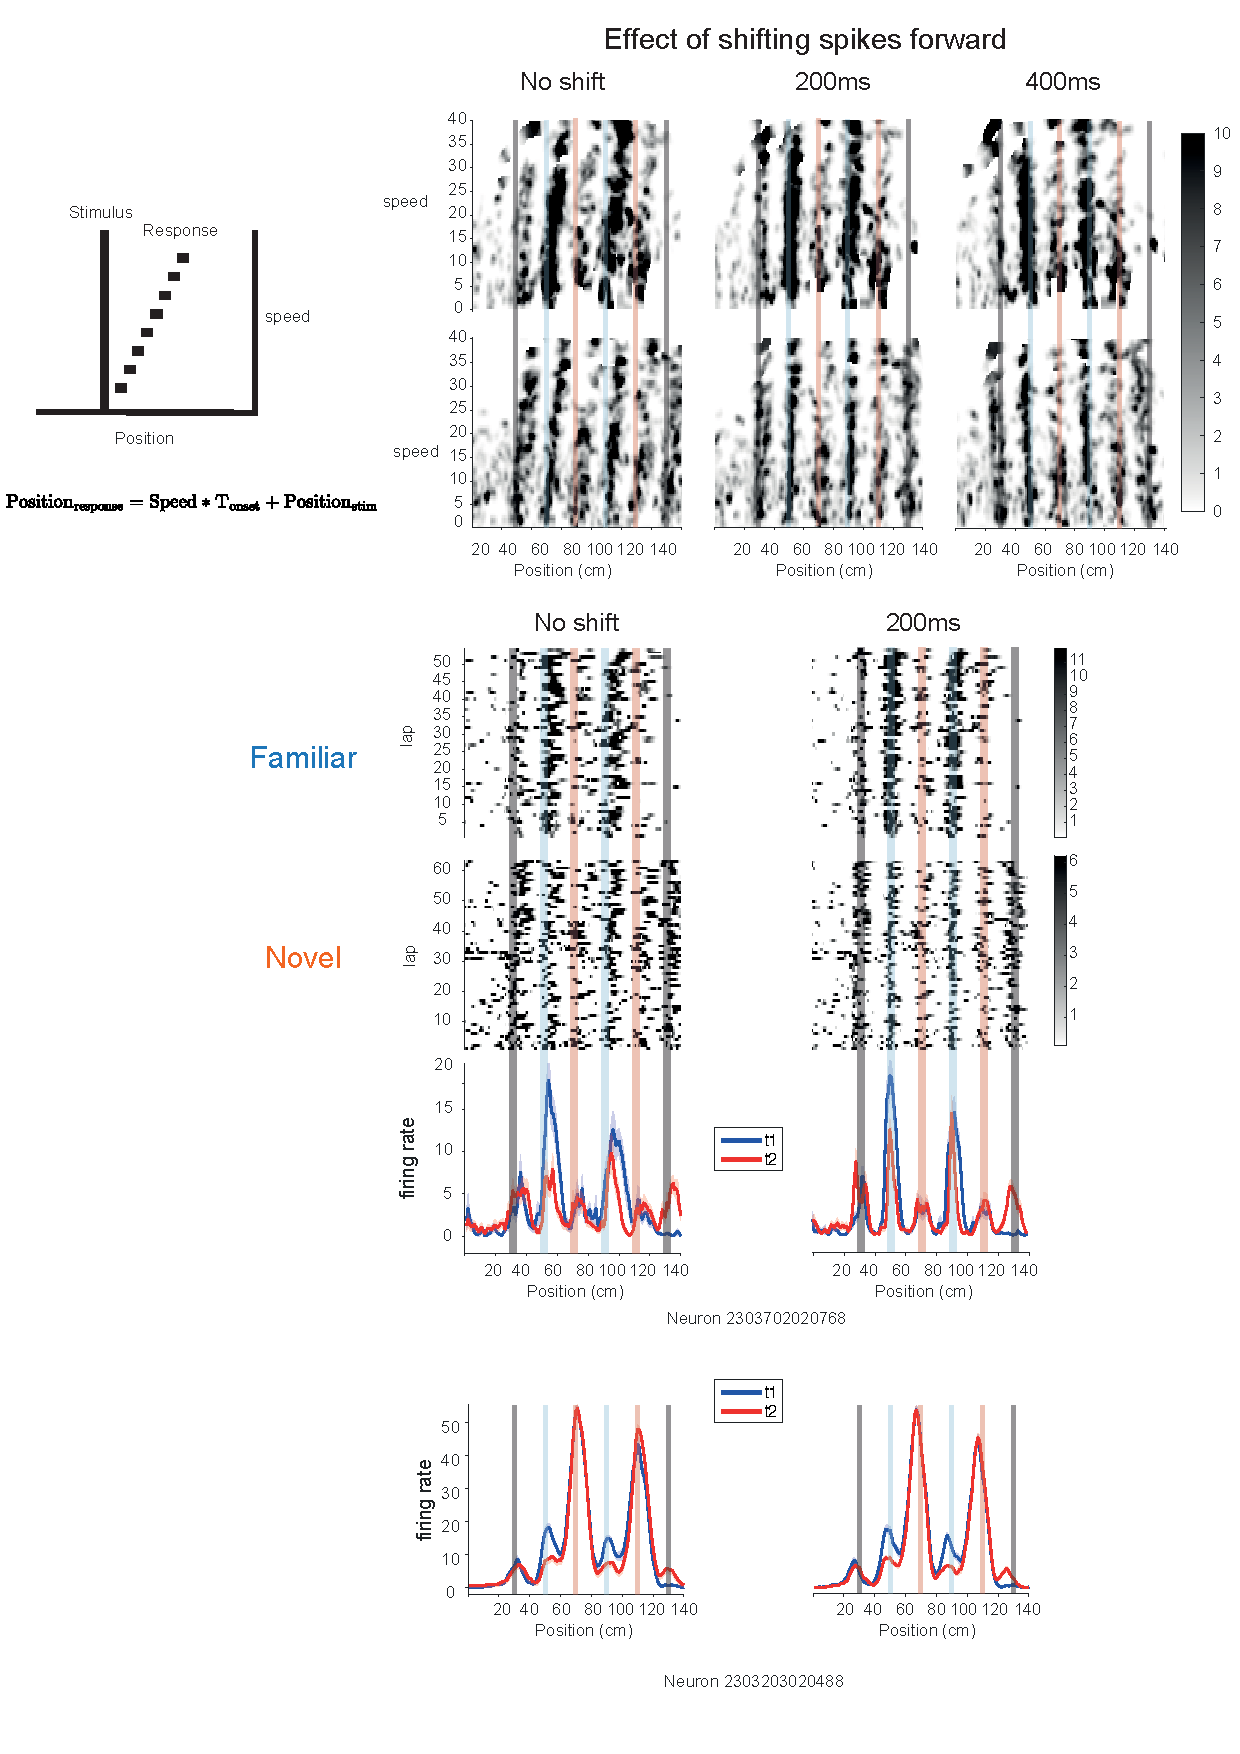
\includegraphics[width=1\linewidth]{figures//Chapter 4 V1/fig2_speed_impact.pdf}
    \caption{Visual cortical responses have delays and their impact on spatial binning depends on the animal's speed in the VR. }
    \label{fig:placeholder}
\end{figure}

\subsection{Spatial Modulation is Present on All Landmarks Across Environments}

\begin{figure}
    \centering
    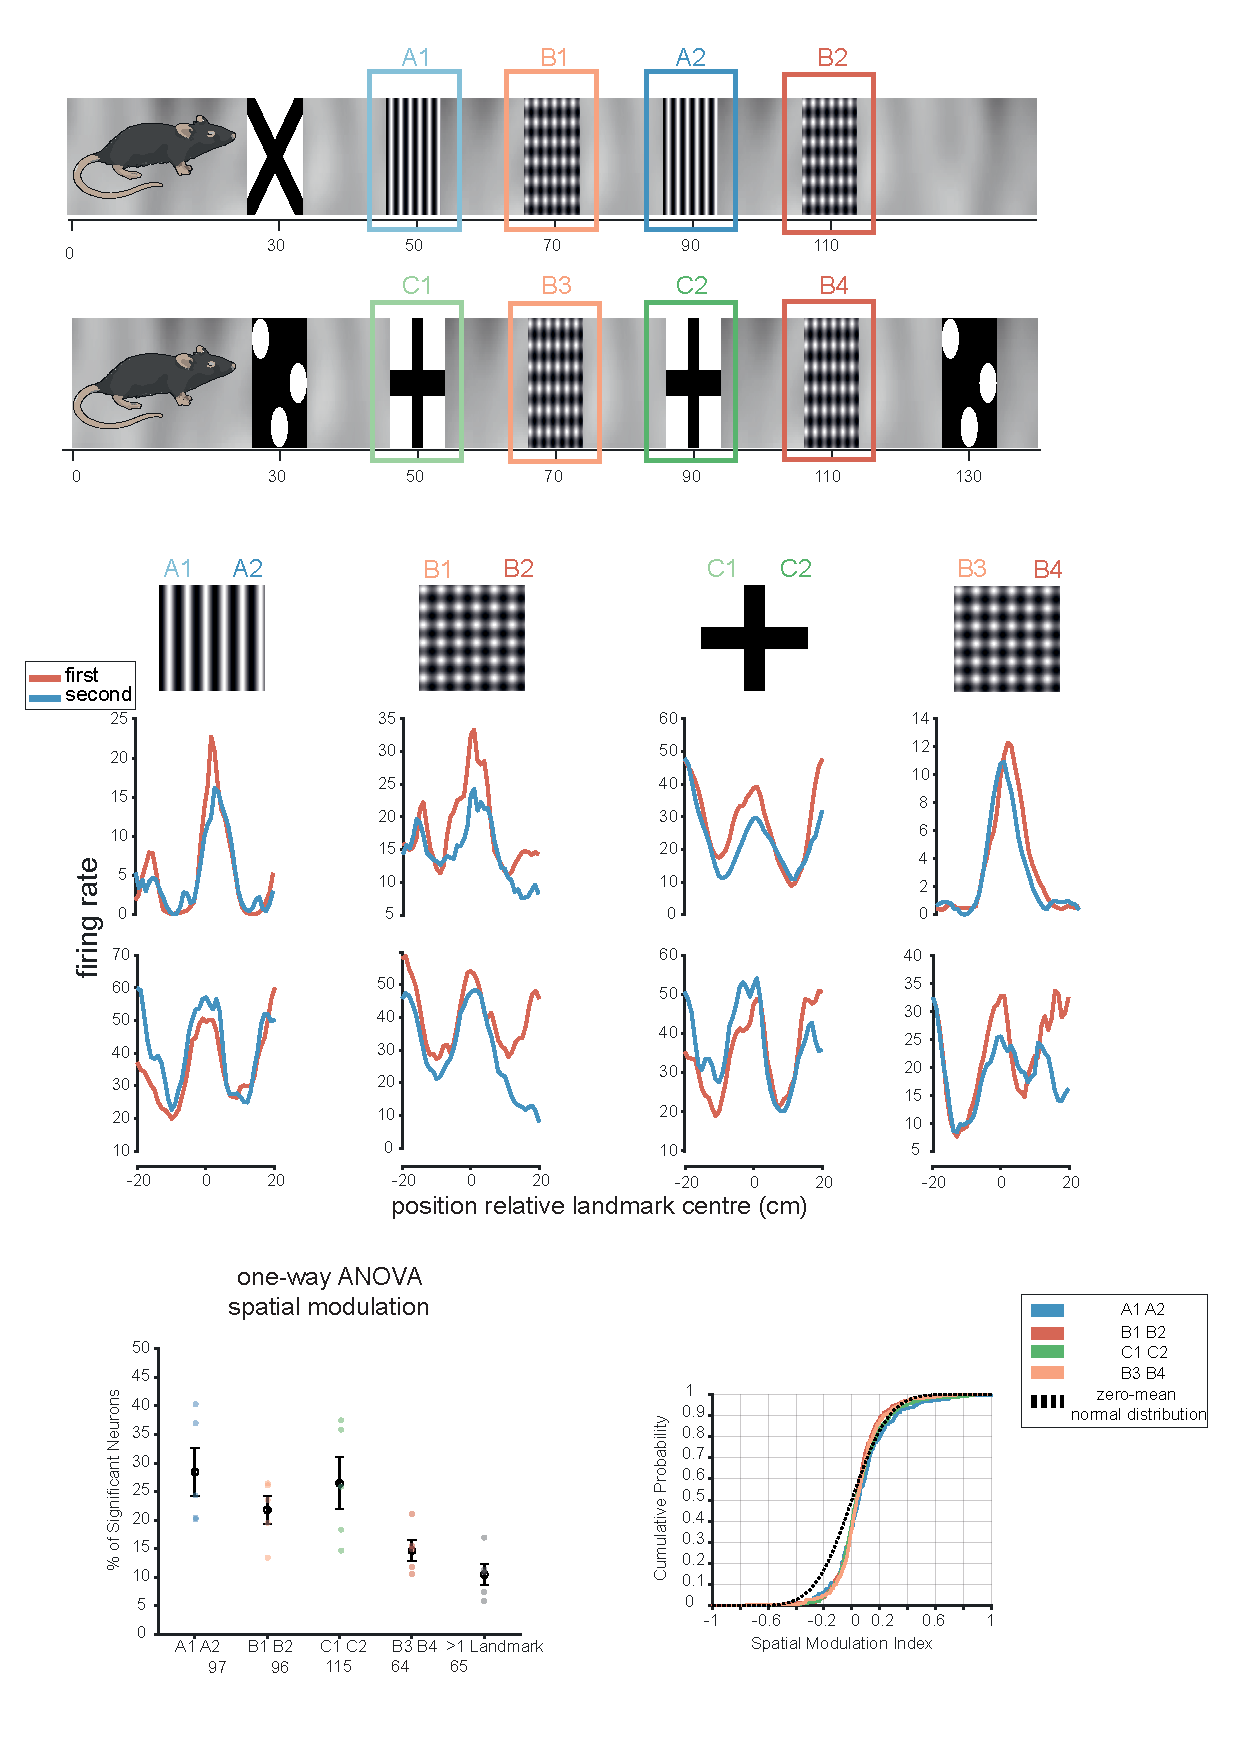
\includegraphics[width=1\linewidth]{figures//Chapter 4 V1/fig3_spatial_modulation_intro.pdf}
    \caption{Spatial modulation on landmark-specific responses in both environments}
    \label{fig:placeholder}
\end{figure}

\subsection{Contextual Modulation Between Two Environments}
\begin{figure}
    \centering
    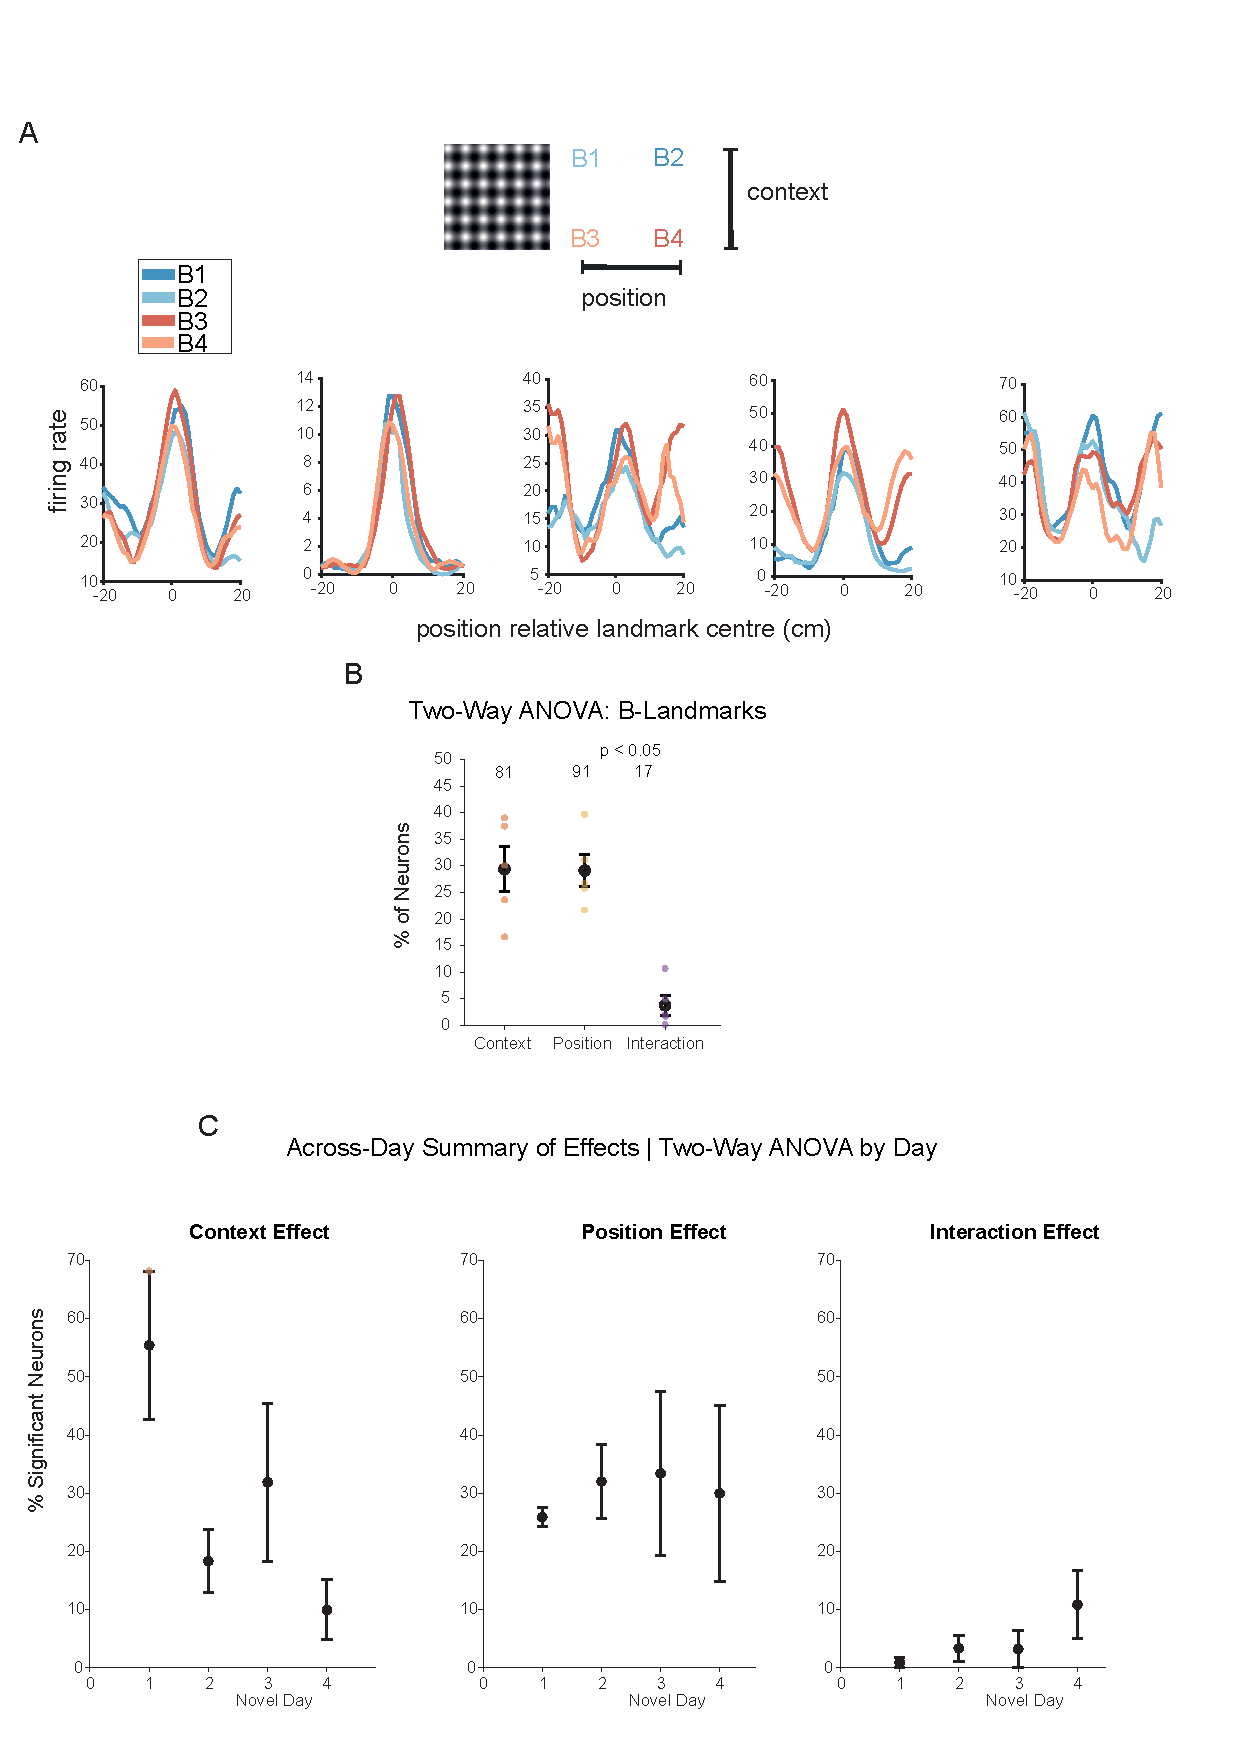
\includegraphics[width=1\linewidth]{figures//Chapter 4 V1/fig4_spatial_modulation_tests.pdf}
    \caption{Spatial and contextual modulations on landmarks shared by both environments. }
    \label{fig:placeholder}
\end{figure}